%Made by Anatolii Anishchenko
%P3112
\newpage
\begin{minipage}[t]{0.25\linewidth}
	\textbf{M329.}
	\textit{Выпуклый n-угольник помещён в квадрат со стороной 1. Докажите,
	что найдётся три вершины A, B, C этого n-угольника такие,
	что площадь треугольника ABC меньше $8/n^2$}
	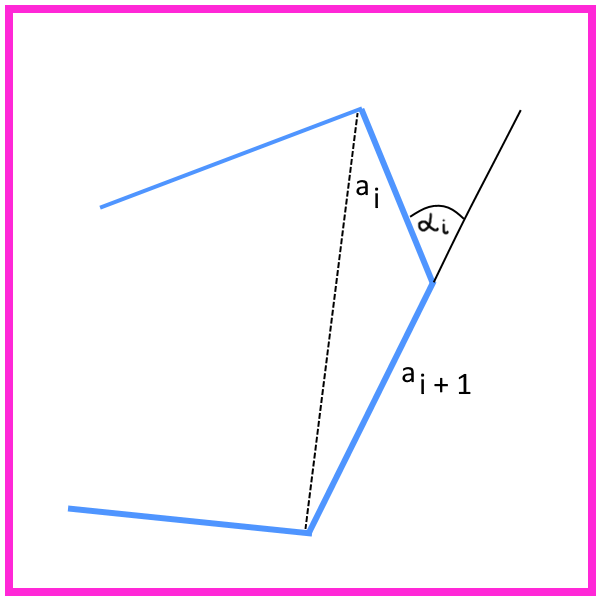
\includegraphics[width=\textwidth]{Lab7.png}
	\hfill
	\textbf{Рис.} 5.
\end{minipage}
\hfill
\begin{minipage}[t]{0.65\linewidth}
	Обозначим через $a_1, a_2, \ldots, a_n$ длины сторон нашего $n$-угольника,
	через $\alpha_1, \ldots, \alpha_n$ -- величины его внутренних углов.
	Пусть $S_i$ -- площадь $i$-того треугольника (со
	сторонами $a_i$ и $a_{i+1}$ -- см. рисунок 5, $i = 1, 2, \ldots, n - 1$),
	$S_n$ -- площадь треугольника со сторонами $a_n, a_1$.
	Имеем: $2S_i=a_ia_{i+1}\sin{\alpha_i}$, $i = 1, 2, \ldots, n - 1$,
	$2S_n=a_na_1\sin{\alpha_n}$.
	Пусть $S$ -- наименьшая из площадей этих треугольников. Тогда
	$$2S \leqslant a_ia_{i+1}\sin{\alpha_i},$$
	откуда
	$$\left(2S\right)^n \leqslant \prod\limits_{i = 1}^n{a_i^2}
	\prod\limits_{i = 1}^n\sin{\alpha_i} < \prod\limits_{i=1}^n{a_i^2}{}^{*}),$$
	то есть
	$$2S < \left(\prod\limits_{i=1}^n{a_i}\right)^{2/n}$$
	Но
	$$\left(\prod\limits_{i}{a_i}\right)^{\frac{1}{n}} = \sqrt[n]
	{a_1 \cdot \ldots \cdot a_n} \leqslant \frac{a_1 + \cdots + a_n}{n}{}^{**})
	= \frac{\sum\limits_{i=1}^n{a_i}}{n},$$
	поэтому
	$$2S < \left({{\sum\limits_{i = 1}^n{a_i}}\over {n}}\right)^2.$$
	Пусть $p_i$ и $q_i$ -- длины проекций $i$-й стороны $n$-угольника на
	вертикальную и горизонтальную стороны квадрата. Тогда $a_i \leqslant
	p_i + q_i$, то есть $\sum\limits_i{a_i} \leqslant \sum\limits_i{p_i} 
	+ \sum\limits_i{q_i} \leqslant 4$
	\newline
	Поэтому
	$$2S < \left(\frac{4}{n}\right)^2,$$
	откуда
	$$S < \frac{8}{n^2}.$$
	\tab Получившаяся оценка довольно груба -- мы с самого начала отбросили
	$\prod\limits_{i=1}^n{\alpha_i}$, оценив это произведение единицей.
	Уточним эту оценку. Имеем:
	$$\left(2S\right)^n \leqslant \prod\limits_{i=1}^n{a_i^2}
	\cdot \prod\limits_{i+1}^n{\alpha_i},$$
	то есть
	$$2S \leqslant \left(\prod\limits_{i=1}^n{a_i}\right)^{2/n}
	\cdot \left(\prod\limits_{i=1}^n{\alpha_i}\right)^{1/n} \leqslant 
	\frac {16} {n^2} \cdot \frac {\sum\limits_{i=1}^n{\sin{\alpha_i}}}{n}.$$
	
	\footnotetext{*) Здесь $\prod\limits_{i}$ -- знак произведения:  
	$\prod\limits_{i=1}^n{a_i}=a_1\cdot \ldots \cdot a_n$.}
	\footnotetext{**) Мы восполользовались неравенством о среднем арифмитическом 
	и среднем геометрическом.}
\end{minipage}

\newpage
Так как я совсем забыл про таблицу, то я вставил её отдельно на следующей стрпнице. 
Заполнив её списком заданий на данную лабораторную работу.
\begin{center}
	\begin{tabular}{|p{4cm}|p{2cm}|p{10cm}|}
		\hline
		\multicolumn{3}{|c|}{Задание} \\
		\hline
		Номер задания & Проценты & Текст задания \\
		\hline
		Обязательно задание & $<= 75\%$ & Сверстать страницу, максимально
		похожую на выбранную страницу из журнала «Квант». \\
		\hline
		Необязательное задание №1 & $+10\%$ & 
		\textit{Выполнение данного задания позволяет получить до 10
		дополнительных баллов.}
		\begin{enumerate}
			\item Сверстать титульный лист
			\item Создать файл \textit{main.tex}, в котором будет
			содержаться преамбула и ссылки на 2 документа: титульный 
			лист и статью (ссылки создаются с помощью команды 
			\textbf{$\backslash$input})
		\end{enumerate}\\
		\hline
		Необязательное задание №2 & $+15\%$ & 
		\textit{Выполнение данного задания позволяет получить до 15 
		дополнительных баллов.}
		\begin{enumerate}
			\item Рассчитать номер варианта по следующей схеме: \newline
			\textit{$N_1$ – количество букв в фамилии, $N_2$ – 
			количество букв в имени}
			\newline \textit{Номер варианта }$= 1 + \left(
			\left(N_1*N_2\right)\mod 8 \right)$
			\item Выполнить задание из полученного варианта, используя
			средства $L^AT_EX$
		\end{enumerate}
		В каждом варианте указаны пакеты или классы документов,
		использование которых необходимо или полезно для выполнения
		задания.\\
		\hline
	\end{tabular}
\end{center}